% MÉTODOS Y MATERIALES

\cleardoublepage

\chapter{Materiales y métodos}

\section{Materiales}

\section{Metodología}

Para el desarrollo de este TFM y del software que lo culminará, se han barajado 3 maneras, \emph{frameworks} o métodos de emprender y encaminar esta labor, de manera rigurosa, estructurada y ordenada. Los nombres que se han manejado han sido:
\begin{itemize}
    \item CRSIP-ML(Q): Cross Industry Standard Process for Machine Learning with Quality Assurance
    \item TDSP: Team Data Science Process
    \item Scrum: del rugby, ideal que significa trabajo en equipo y rápida respuesta de adaptación.
\end{itemize}

Cada una de estas tres herramientas aporta valor a cada uno de los pasos que se puedan llevar a cabo. Haciendo un análisis más profundo y tal y como se explica en la entrada web\cite{TDSP-PM}, se podría decir que \emph{TDSP} podría ser la combinación de \emph{Scrum} y \emph{CRISP-DM} (Cross Industry Standard Process for Data Mining. En el caso de proyectos de Machine Learning, CRISP-ML(Q) parte de la misma filosfía y se adapta a las necesidades específicas de este tipo de trabjos). Así pues, dado que todo lo referente a gestión de equipo y recursos en paralelo es innecesario, pues este trabajo se realiza por una sola persona, se ha decidido tomar un combinación de \textbf{CRISP-ML(Q)} y \textbf{Scrum}, que permita ser tan riguroso como el primero de ellos y tan ágil y potente en cuanto a herramientas, como el segundo.

\subsection{CRISP-ML(Q)}

\emph{CRISP-ML(Q)} conforma un marco estructurado para el desarrollo de proyectos de Machine Learning. Se compone de seis fases:

\begin{enumerate}
    \item \textbf{Comprensión del negocio}: Definir el problema y los objetivos del modelo.
    \item \textbf{Comprensión de los datos}: Recopilación y exploración inicial de los datos.
    \item \textbf{Preparación de los datos}: Limpieza, transformación y selección de variables.
    \item \textbf{Modelado}: Entrenamiento y optimización de modelos de Machine Learning.
    \item \textbf{Evaluación}: Validación de métricas y análisis del rendimiento.
    \item \textbf{Implementación y monitoreo}: Despliegue del modelo y seguimiento en producción.
\end{enumerate}

\begin{figure}[H]
  \centering
  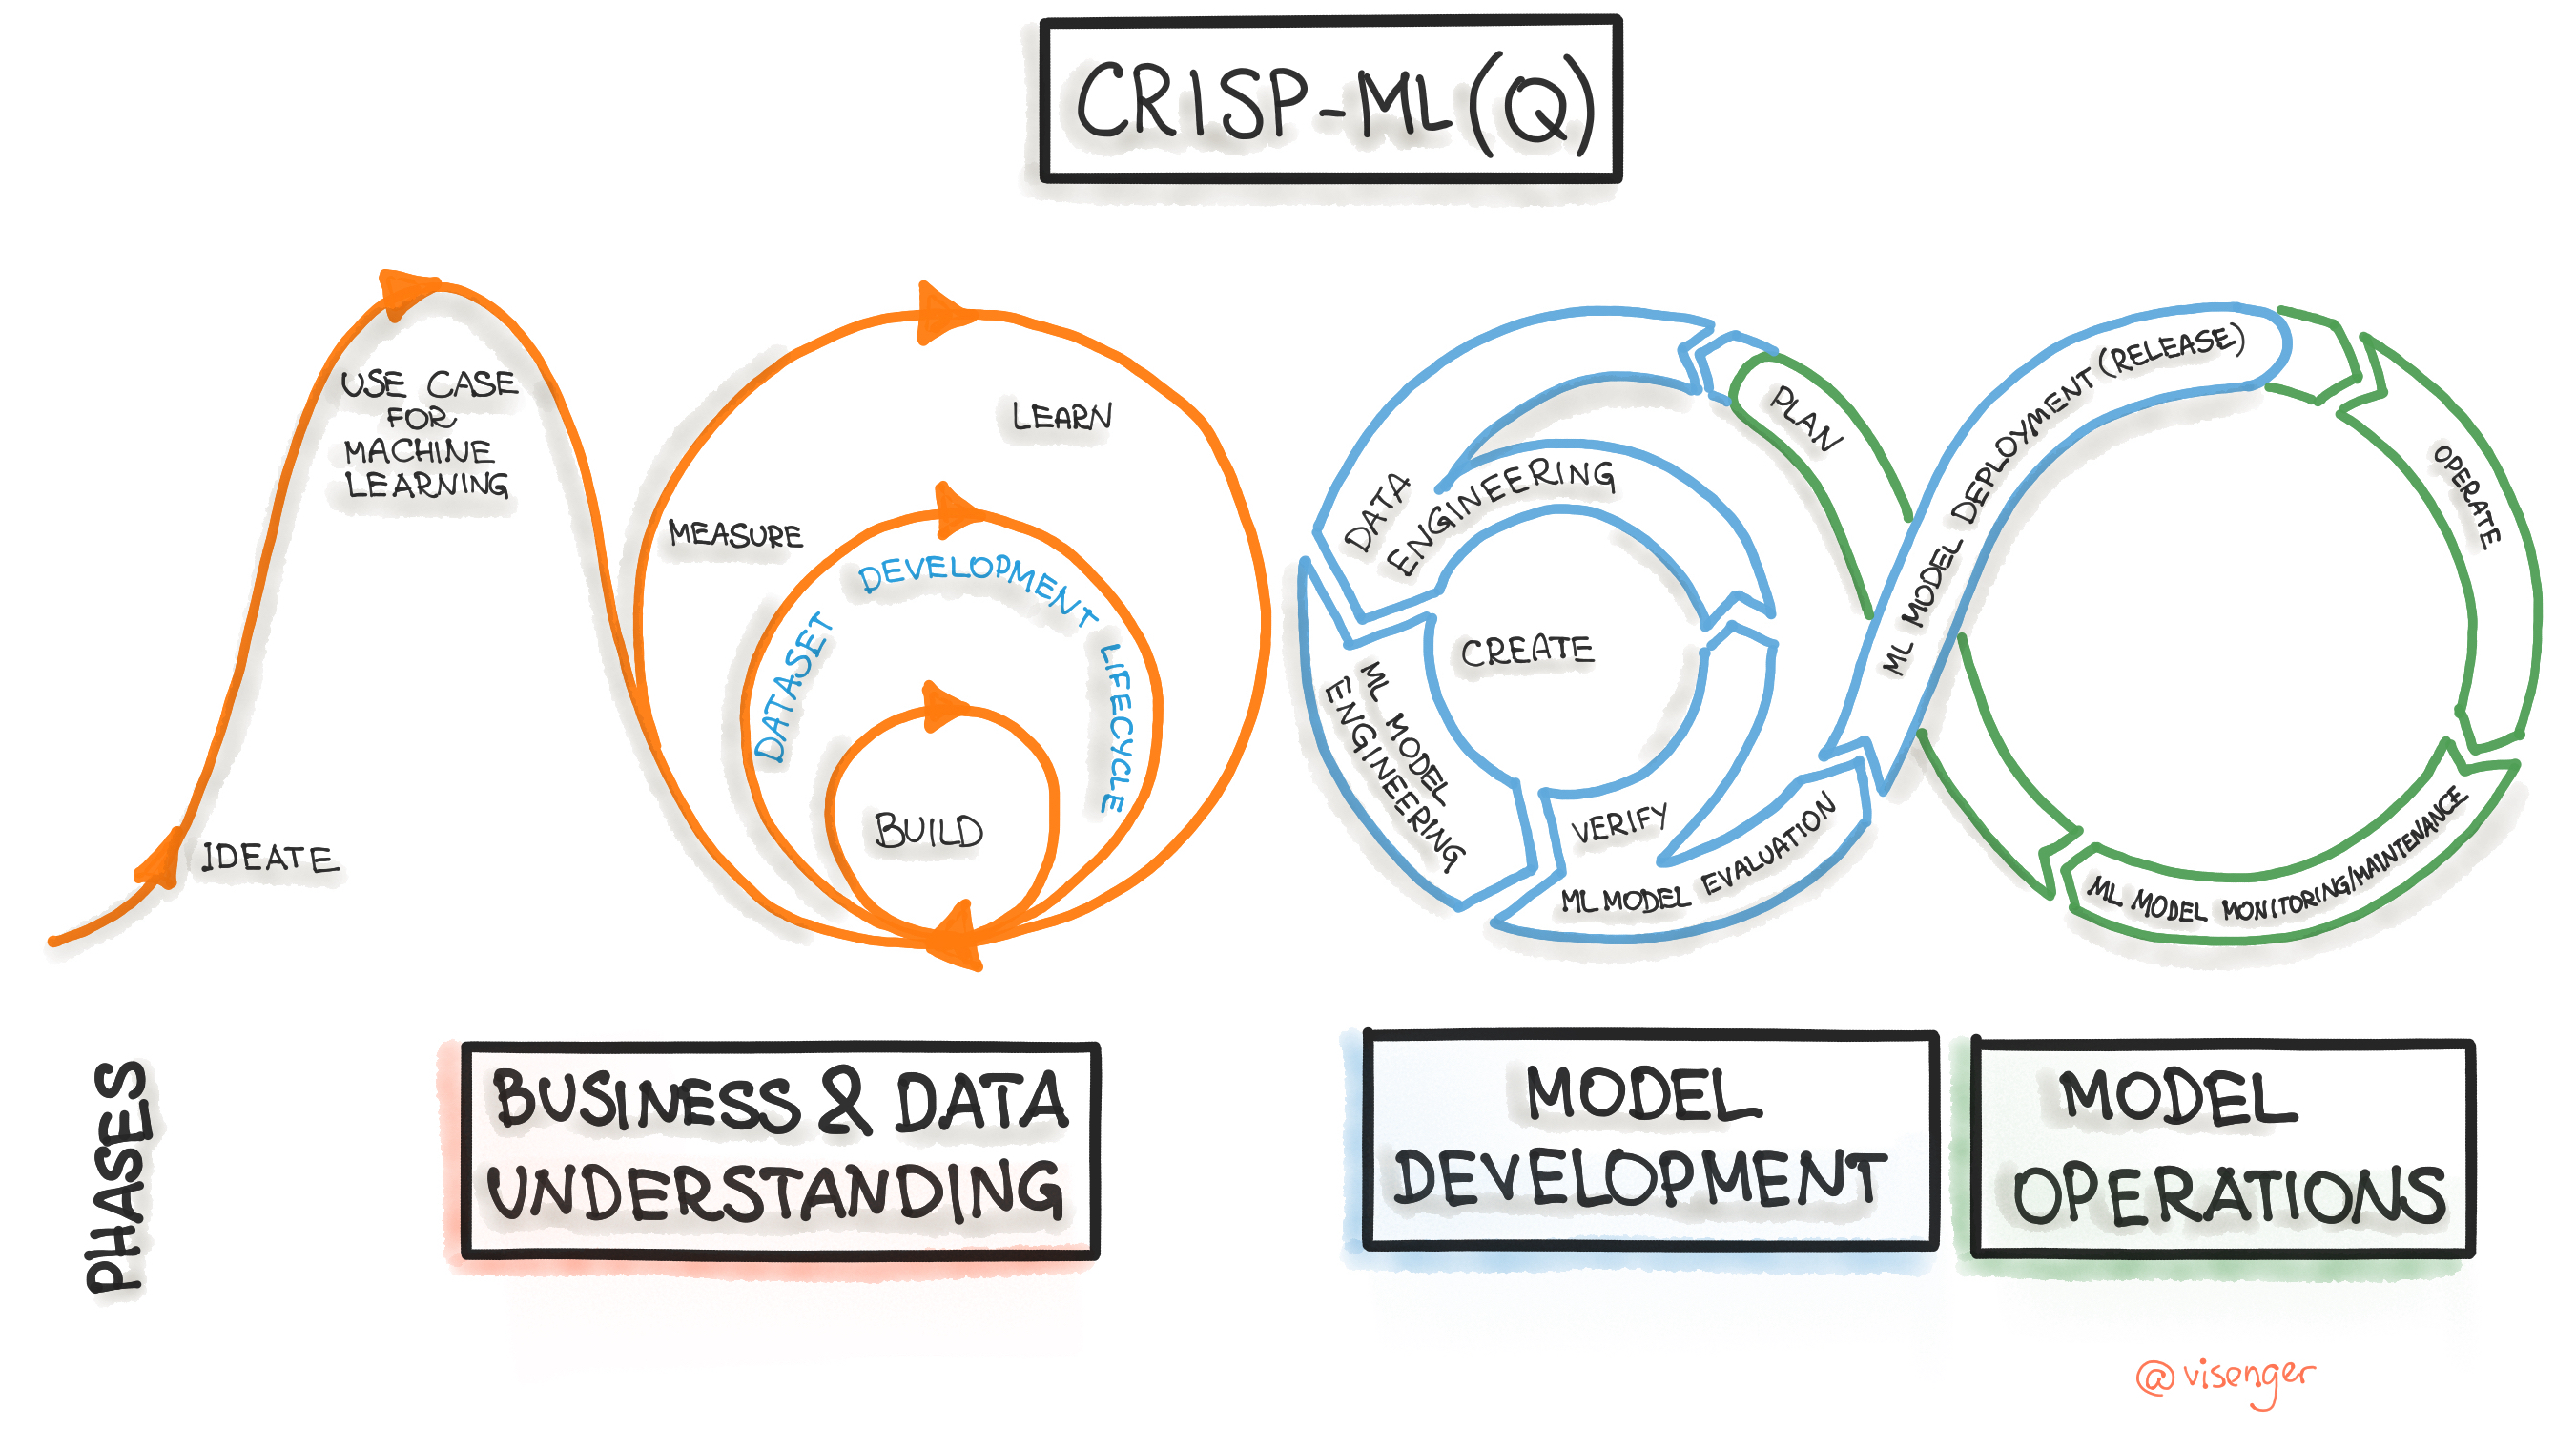
\includegraphics[width=0.9\textwidth]{images/crisp-ml-process.jpg}
  \caption{Diagrama de flujo usado en el desarrollo. Tomado de \cite{crispml}.}
  \label{fig:crispml-q-diagram}
\end{figure}

En la imagen\cite{crispml-q-diagram} se puede ver cómo será el diagrama de flujo del desarrollo a seguir con este método.

\subsection{Scrum}

\emph{Scrum} es un framework que proporciona herramientas para la gestión ágil de proyectos de manera iterativa, dividiendo el trabajo en sprints (iteraciones cortas de 1-2 semanas). Las herramientas de \emph{Scrum} que se tomen para este proyecto serán:

\begin{itemize}
    \item \textbf{Product Backlog}: Lista priorizada de tareas a realizar.
    \item \textbf{Sprints}: Iteraciones donde se completan tareas específicas. Semanales.
    \item \textbf{Sprint Reviews}: Evaluaciones de cada sprint (semana o bisemanal) con la tutora de este TFM.
\end{itemize}

\subsection{Integración de CRISP-ML(Q) y Scrum}

A continuación, se detalla la planificación del TFM en base a estos marcos metodológicos.

\subsection{Product Backlog}

Las tareas que se han de llevar a cabo para completar el TFM, incluidos desarrollo de la documentación, software y evaluación y mantenimiento, se han organizado en el siguiente \emph{backlog}:

% \begin{table}[h]
%     \centering
    
%     \resizebox{\textwidth}{!}{
%     \begin{tabular}{|c|c|p{8cm}|c|}
%         \hline
%         \textbf{Épica} & \textbf{Historia de Usuario} & \textbf{Tareas} & \textbf{Prioridad} \\
%         \hline
%         Comprensión del negocio & Definir el problema & Redactar introducción, revisar 10 artículos, definir impacto y KPIs & Alta \\
%         \hline
%         Comprensión de los datos & Analizar calidad de los datos & Inspeccionar valores nulos, outliers, generar gráficos EDA & Alta \\
%         \hline
%         Preparación de los datos & Preprocesamiento de datos & Normalizar, codificar variables, dividir en train/test & Media \\
%         \hline
%         Modelado & Entrenar modelos de ML & Implementar baseline, probar algoritmos, ajustar hiperparámetros & Alta \\
%         \hline
%         Evaluación & Validar rendimiento del modelo & Comparar métricas, generar reportes de resultados & Alta \\
%         \hline
%         Implementación y monitoreo & Redactar el TFM & Documentar metodología, resultados, preparar presentación & Alta \\
%         \hline
%     \end{tabular}}
% \end{table}

\begin{table}[h]
    \centering
    \caption{Product Backlog (Pila de producto) del TFM basado en CRISP-ML(Q) y Scrum}
    \resizebox{0.8\textwidth}{!}{
    \begin{tabular}{|c|p{8cm}|p{8cm}|}
        \hline
        \textbf{Épica (Fase CRISP-ML(Q))} & \textbf{Historia de Usuario} & \textbf{Tareas} \\
        \hline
        Comprensión del negocio &  Como estudiante, quiero comprender bien el problema para entender el alcance del proyecto. & 
        \begin{itemize}
            \item Redactar introducción.
            \item Definir objetivos generales y específicos.
            \item Entender y tomar notas sobre el alcance del proyecto.
        \end{itemize} \\
        \hline
        Comprensión del negocio & Como estudiante, en mi labor de investigación, quiero revisar literatura existente en torno al problema.  &
        \begin{itemize}
            \item Buscar y analizar artículos y publicaciones relevantes. 
            \item Extraer ideas clave.
            \item Identificar tendencias en el estado del arte.
        \end{itemize} \\
        \hline
        Comprensión de los datos & Como estudiante, emulando a un científico de datos, quiero inspeccionar los datos disponibles para evaluar su calidad. & 
        \begin{itemize}
            \item Encontrar fuentes con datasets adecuados.
            \item Revisar estructura y tipos de datos.
            \item Evaluar insuficiencia, sesgo o desbalanceo en los datos.
            \item Escribir la metodología detallada.
        \end{itemize} \\
        \hline
        Preparación de los datos & Como estudiante y desarrollador, quiero limpiar y transformar los datos para que sean aptos para el modelo. & 
        \begin{itemize}
            \item Normalizar y codificar variables.
            \item Manejar valores atípicos y nulos.
        \end{itemize} \\
        \hline
        Preparación de los datos & Como estudiante y desarrollador, quiero dividir los datos en conjuntos de entrenamiento, validación y prueba. & 
        \begin{itemize}
            \item Definir proporción de separación de datos.
            \item Verificar balanceo de clases.
        \end{itemize} \\
        \hline
        Modelado & Como estudiante, emulando a un científico de datos, quiero entrenar un modelo base para establecer un punto de comparación. & 
        \begin{itemize}
            \item Entrenar el VAE.
            \item Evaluar rendimiento inicial.
            \item Extraer los primeros resultados.
        \end{itemize} \\
        \hline
        Modelado & Como estudiante, emulando a un científico de datos, quiero entrenar un modelo basado en GAN-Transformer y evaluar su precisión. & 
        \begin{itemize}
            \item Implementar y entrenar el modelo GAN-Transformer.
            \item Comparar modelos con métricas clave.
        \end{itemize} \\
        \hline
        Evaluación & Como estudiante e investigador, quiero evaluar el rendimiento del modelo para justificar su efectividad. &
        \begin{itemize}
            \item Calcular precisión, recall y F1-score.
            \item Generar matriz de confusión.
            \item Comparar modelos.
        \end{itemize} \\
        \hline
        Evaluación & Como estudiante e investigador, quiero establecer métricas comparativas entre los enfoques y mejorar la red GAN. & 
        \begin{itemize}
            \item Analizar interpretabilidad de los resultados.
            \item Ajustar hiperparámetros y arquitectura.
        \end{itemize} \\
        \hline
        Implementación y monitoreo & Como estudiante, quiero documentar la metodología utilizada para su presentación y evaluación. & 
        \begin{itemize}
            \item Documentar pruebas de los modelos.
            \item Preparar informe técnico.
        \end{itemize} \\
        \hline
        Implementación y monitoreo & Como estudiante, quiero preparar una presentación clara y concisa para la defensa del TFM. & 
        \begin{itemize}
            \item Diseñar diapositivas con gráficos y métricas.
            \item Exponer conclusiones.
            \item Practicar la presentación.
        \end{itemize} \\
        \hline
    \end{tabular}}
\end{table}


\clearpage
\begin{tcolorbox}[colback=black!85!white, colframe=orange!60!black, fontupper=\color{white},
    title=\textbf{\huge Product Backlog (Pila de producto)}, fonttitle=\color{white}]
    
        \begin{center}
        \renewcommand{\arraystretch}{0.2} % Reduce la separación entre filas
        \setlength{\tabcolsep}{8pt} % Reduce la separación entre columnas
        \resizebox{0.8\textwidth}{!}{ % Ajusta la tabla al 95% del ancho del texto
        \begin{tabular}{m{0.32\textwidth}<{\raggedright} m{0.32\textwidth}<{\raggedright} m{0.32\textwidth}<{\raggedright}} % 3 COLUMNAS BALANCEADAS
        
            %%%% FILA 1 - Comprensión del negocio (CN)
            \begin{tcolorbox}[colback=yellow!70!white, colframe=yellow!90!white, title={\textbf{CN-1}}, fonttitle=\color{black}]
            Redactar introducción.
            \end{tcolorbox} &        
            \begin{tcolorbox}[colback=yellow!70!white, colframe=yellow!90!white, title={\textbf{CN-2}}, fonttitle=\color{black}]
            Definir objetivos generales y específicos.
            \end{tcolorbox} &        
            \begin{tcolorbox}[colback=yellow!70!white, colframe=yellow!90!white, title={\textbf{CN-3}}, fonttitle=\color{black}]
            Entender y tomar notas sobre el alcance del proyecto.
            \end{tcolorbox} \\
    
            %%%% FILA 2
            \begin{tcolorbox}[colback=yellow!70!white, colframe=yellow!90!white, title={\textbf{CN-4}}, fonttitle=\color{black}]
            Buscar y analizar artículos y publicaciones relevantes.
            \end{tcolorbox} &
            \begin{tcolorbox}[colback=yellow!70!white, colframe=yellow!90!white, title={\textbf{CN-5}}, fonttitle=\color{black}]
            Extraer ideas clave.
            \end{tcolorbox} &
            \begin{tcolorbox}[colback=yellow!70!white, colframe=yellow!90!white, title={\textbf{CN-6}}, fonttitle=\color{black}]
            Identificar tendencias en el estado del arte.
            \end{tcolorbox} \\
    
            %%%% FILA 3 - Comprensión de los datos (CD)
            \begin{tcolorbox}[colback=purple!30!white, colframe=purple!40!white, title={\textbf{CD-1}}, fonttitle=\color{black}]
            Encontrar fuentes con datasets adecuados.
            \end{tcolorbox} &
            \begin{tcolorbox}[colback=purple!30!white, colframe=purple!40!white, title={\textbf{CD-2}}, fonttitle=\color{black}]
            Revisar estructura y tipos de datos.
            \end{tcolorbox} &
            \begin{tcolorbox}[colback=purple!30!white, colframe=purple!40!white, title={\textbf{CD-3}}, fonttitle=\color{black}]
            Evaluar insuficiencia, sesgo o desbalanceo en los datos.
            \end{tcolorbox} \\
    
            %%%% FILA 4
            \begin{tcolorbox}[colback=purple!30!white, colframe=purple!40!white, title={\textbf{CD-4}}, fonttitle=\color{black}]
            Escribir la metodología detallada.
            \end{tcolorbox} &
            \begin{tcolorbox}[colback=green!50!yellow, colframe=green!80!yellow, title={\textbf{PD-1}}, fonttitle=\color{black}]
            Normalizar y codificar variables.
            \end{tcolorbox} &
            \begin{tcolorbox}[colback=green!50!yellow, colframe=green!80!yellow, title={\textbf{PD-2}}, fonttitle=\color{black}]
            Manejar valores atípicos y nulos.
            \end{tcolorbox} \\
            \begin{tcolorbox}[colback=green!50!yellow, colframe=green!80!yellow, title={\textbf{PD-3}}, fonttitle=\color{black}]
            Definir proporción de separación de datos.
            \end{tcolorbox} &
    
            %%%% FILA 5
            \begin{tcolorbox}[colback=green!50!yellow, colframe=green!80!yellow, title={\textbf{PD-4}}, fonttitle=\color{black}]
            Verificar balanceo de clases.
            \end{tcolorbox} &
            \begin{tcolorbox}[colback=pink!60!red, colframe=pink!40!red, title={\textbf{M-1}}, fonttitle=\color{black}]
            Entrenar el VAE.
            \end{tcolorbox} \\
            \begin{tcolorbox}[colback=pink!60!red, colframe=pink!40!red, title={\textbf{M-2}}, fonttitle=\color{black}]
            Evaluar rendimiento inicial.
            \end{tcolorbox} &
    
            %%%% FILA 6
            \begin{tcolorbox}[colback=pink!60!red, colframe=pink!40!red, title={\textbf{M-3}}, fonttitle=\color{black}]
            Extraer los primeros resultados.
            \end{tcolorbox} &
            \begin{tcolorbox}[colback=pink!60!red, colframe=pink!40!red, title={\textbf{M-4}}, fonttitle=\color{black}]
            Implementar y entrenar el modelo GAN-Transformer.
            \end{tcolorbox} \\
            
            \begin{tcolorbox}[colback=pink!60!red, colframe=pink!40!red, title={\textbf{M-5}}, fonttitle=\color{black}]
            Comparar modelos con métricas clave.
            \end{tcolorbox} &
            \begin{tcolorbox}[colback=orange!70!white, colframe=orange!90!white, title={\textbf{EV-1}}, fonttitle=\color{black}]
            Calcular precisión, recall y F1-score.
            \end{tcolorbox} &
            \begin{tcolorbox}[colback=orange!70!white, colframe=orange!90!white, title={\textbf{EV-2}}, fonttitle=\color{black}]
            Generar matriz de confusión.
            \end{tcolorbox}
            \\

            %%%% FILA 8
            \begin{tcolorbox}[colback=orange!70!white, colframe=orange!90!white, title={\textbf{EV-3}}, fonttitle=\color{black}]
                Comparar modelos.
                
                \end{tcolorbox}
            &
            
            \begin{tcolorbox}[colback=orange!70!white, colframe=orange!90!white, title={\textbf{EV-4}}, fonttitle=\color{black}]
                Analizar interpretabilidad de los resultados.
                \end{tcolorbox} &

                \begin{tcolorbox}[colback=orange!70!white, colframe=orange!90!white, title={\textbf{EV-5}}, fonttitle=\color{black}]
                    Ajustar hiperparámetros y arquitectura.
                    \end{tcolorbox} 

            \\
    
            %%%% FILA 9
            
            \begin{tcolorbox}[colback=blue!30!white, colframe=blue!40!white, title={\textbf{IM-1}}, fonttitle=\color{black}]
            Documentar pruebas de los modelos.
            \end{tcolorbox} &
            \begin{tcolorbox}[colback=blue!30!white, colframe=blue!40!white, title={\textbf{IM-2}}, fonttitle=\color{black}]
            Preparar informe técnico.
            \end{tcolorbox} &
    
            %%%% FILA 10
            \begin{tcolorbox}[colback=blue!30!white, colframe=blue!40!white, title={\textbf{IM-3}}, fonttitle=\color{black}]
            Diseñar diapositivas con gráficos y métricas.
            \end{tcolorbox} \\
            \begin{tcolorbox}[colback=blue!30!white, colframe=blue!40!white, title={\textbf{IM-4}}, fonttitle=\color{black}]
            Exponer conclusiones.
            \end{tcolorbox} &
            \begin{tcolorbox}[colback=blue!30!white, colframe=blue!40!white, title={\textbf{IM-5}}, fonttitle=\color{black}]
            Practicar la presentación.
            \end{tcolorbox} \\
    
        \end{tabular}
        }
        \end{center}
    
    \end{tcolorbox}
    
\clearpage
\begin{table}[h]
    \centering
    \caption{Kanban del TFM basado en CRISP-ML(Q) y Scrum}
    \resizebox{\textwidth}{!}{
    \begin{tabular}{|p{8cm}|c|p{2.5cm}|}
        \hline
        \textbf{Tarea} & \textbf{Categoría\hfill \break CRISP-ML(Q) / (Código)} & \textbf{Estado} \\
        \hline
        Definir problema del TFM & Comprensión del negocio / (CN-1)& \ding{51}Hecho \\
        \hline
        Revisar al menos 10 artículos & Comprensión del negocio / (CN-2)& \ding{51}Hecho \\
        \hline
        Definir métricas clave (KPIs) & Comprensión del negocio / (CN-3)& \ding{51}Hecho \\
        \hline
        Recopilar datasets disponibles & Comprensión de los datos / (CD-1)& \ding{51}Hecho \\
        \hline
        Realizar análisis exploratorio (EDA) & Comprensión de los datos / (CD-2)&\ding{51}Hecho \\
        \hline
        Identificar valores nulos y outliers & Comprensión de los datos / (CD-3)&\ding{45}En progreso \\
        \hline
        Generar visualización de datos & Comprensión de los datos / (CD-4)& \ding{51}Hecho \\
        \hline
        Limpieza y preprocesamiento de datos & Preparación de los datos / (PD-1) & \ding{45}En progreso \\
        \hline
        Normalización y codificación de variables & Preparación de los datos / (PD-2) &\ding{43}Por hacer \\
        \hline
        Dividir dataset en train/val/test & Preparación de los datos / (PD-3) &\ding{43}Por hacer \\
        \hline
        Implementar modelo base (benchmark) & Modelado / (M-1) & \ding{43}Por hacer \\
        \hline
        Probar al menos 2-3 modelos & Modelado / (M-2) & \ding{43}Por hacer \\
        \hline
        Ajustar hiperparámetros & Modelado / (M-3) &\ding{43}Por hacer \\
        \hline
        Comparar métricas de rendimiento & Evaluación / (Ev-1) &\ding{43}Por hacer \\
        \hline
        Generar matriz de confusión & Evaluación / (Ev-2) &\ding{43}Por hacer \\
        \hline
        Documentar los resultados & Evaluación / (Ev-3) &\ding{43}Por hacer \\
        \hline
        Preparar presentación final & Implementación y monitoreo / (IM-1) &\ding{43}Por hacer \\
        \hline
    \end{tabular}}
\end{table}
\newpage
\begin{tcolorbox}[colback=black!85!white, colframe=orange!60!black, fontupper=\color{white},
    title=\textbf{\huge Kanban}, fonttitle=\color{white}]
    {\huge \emph{Sprint 3}}
        \begin{center}
            \renewcommand{\arraystretch}{0.2} % Reduce la separación entre filas
            \setlength{\tabcolsep}{8pt} % Reduce la separación entre columnas
            \resizebox{\textwidth}{!}{ % Ajusta la tabla al 95% del ancho del texto
            \begin{tabular}{m{4cm} m{4cm} m{4cm} m{4cm} m{4cm}}
            \begin{center}
            {\Fontauri \huge \emph{to do}}
            \end{center}
            & \begin{center}
            {\Fontauri \huge \emph{to do}} 
            \end{center}
            & \begin{center}
            {\Fontauri \huge \emph{to do}} 
            \end{center}
            & \begin{center}
            {\Fontauri \huge \emph{in progress}} 
            \end{center} 
            & \begin{center}
            {\Fontauri \huge \emph{done}} 
            \end{center} \\
            
            \begin{tcolorbox}[colback=green!50!white, colframe=green!80!black, title={\textbf{PD-1}}, fonttitle=\color{black}]
            Normalizar y codificar variables.
            \end{tcolorbox} &
            \begin{tcolorbox}[colback=green!50!white, colframe=green!80!black, title={\textbf{PD-2}}, fonttitle=\color{black}]
            Manejar valores atípicos y nulos.
            \end{tcolorbox} &
            \begin{tcolorbox}[colback=green!50!white, colframe=green!80!black, title={\textbf{PD-3}}, fonttitle=\color{black}]
            Definir proporción de separación de datos.
            \end{tcolorbox} &
            \begin{tcolorbox}[colback=purple!30!white, colframe=purple!40!white, title={\textbf{CD-3}}, fonttitle=\color{black}]
            Evaluar insuficiencia, sesgo o desbalanceo en los datos.
            \end{tcolorbox} &
            \begin{tcolorbox}[colback=yellow!70!white, colframe=yellow!90!white, title={\textbf{CN-1}}, fonttitle=\color{black}]
            Redactar introducción.
            \end{tcolorbox}
            \\

            \begin{tcolorbox}[colback=green!50!white, colframe=green!80!black, title={\textbf{PD-4}}, fonttitle=\color{black}]
            Verificar balanceo de clases.
            \end{tcolorbox} &
            \begin{tcolorbox}[colback=pink!60!red, colframe=pink!40!red, title={\textbf{M-1}}, fonttitle=\color{black}]
            Entrenar el VAE.
            \end{tcolorbox} &
            \begin{tcolorbox}[colback=pink!60!red, colframe=pink!40!red, title={\textbf{M-2}}, fonttitle=\color{black}]
            Evaluar rendimiento inicial.
            \end{tcolorbox} &
            &
            \begin{tcolorbox}[colback=yellow!70!white, colframe=yellow!90!white, title={\textbf{CN-2}}, fonttitle=\color{black}]
            Definir objetivos generales y específicos.
            \end{tcolorbox}
            \\
            
            \begin{tcolorbox}[colback=pink!60!red, colframe=pink!40!red, title={\textbf{M-3}}, fonttitle=\color{black}]
            Extraer los primeros resultados.
            \end{tcolorbox} & 
            \begin{tcolorbox}[colback=pink!60!red, colframe=pink!40!red, title={\textbf{M-4}}, fonttitle=\color{black}]
            Implementar y entrenar el modelo GAN-Transformer.
            \end{tcolorbox} &
            \begin{tcolorbox}[colback=pink!60!red, colframe=pink!40!red, title={\textbf{M-5}}, fonttitle=\color{black}]
            Comparar modelos con métricas clave.
            \end{tcolorbox} &
            & 
            \begin{tcolorbox}[colback=yellow!70!white, colframe=yellow!90!white, title={\textbf{CN-3}}, fonttitle=\color{black}]
            Entender y tomar notas sobre el alcance del proyecto.
            \end{tcolorbox} 
            \\

            \begin{tcolorbox}[colback=orange!70!white, colframe=orange!90!white, title={\textbf{EV-1}}, fonttitle=\color{black}]
            Analizar interpretabilidad de los resultados.
            \end{tcolorbox} & 
            \begin{tcolorbox}[colback=orange!70!white, colframe=orange!90!white, title={\textbf{EV-2}}, fonttitle=\color{black}]
            Calcular precisión, recall y F1-score.
            \end{tcolorbox} &
            \begin{tcolorbox}[colback=orange!70!white, colframe=orange!90!white, title={\textbf{EV-3}}, fonttitle=\color{black}]
            Generar matriz de confusión.
            \end{tcolorbox} &
            &
            \begin{tcolorbox}[colback=yellow!70!white, colframe=yellow!90!white, title={\textbf{CN-4}}, fonttitle=\color{black}]
            Buscar y analizar artículos y publicaciones relevantes.
            \end{tcolorbox}    
            \\
    
            
            \begin{tcolorbox}[colback=orange!70!white, colframe=orange!90!white, title={\textbf{EV-4}}, fonttitle=\color{black}]
            Comparar modelos.
            \end{tcolorbox} &
            \begin{tcolorbox}[colback=orange!70!white, colframe=orange!90!white, title={\textbf{EV-5}}, fonttitle=\color{black}]
            Ajustar hiperparámetros y arquitectura.
            \end{tcolorbox} &
            \begin{tcolorbox}[colback=blue!30!white, colframe=blue!40!white, title={\textbf{IM-1}}, fonttitle=\color{black}]
            Documentar pruebas de los modelos.
            \end{tcolorbox} &
            &
            \begin{tcolorbox}[colback=yellow!70!white, colframe=yellow!90!white, title={\textbf{CN-5}}, fonttitle=\color{black}]
            Extraer ideas clave.
            \end{tcolorbox} 
            \\
            
            \begin{tcolorbox}[colback=blue!30!white, colframe=blue!40!white, title={\textbf{IM-2}}, fonttitle=\color{black}]
            Preparar informe técnico.
            \end{tcolorbox} &
            \begin{tcolorbox}[colback=blue!30!white, colframe=blue!40!white, title={\textbf{IM-3}}, fonttitle=\color{black}]
            Diseñar diapositivas con gráficos y métricas.
            \end{tcolorbox} &
            \begin{tcolorbox}[colback=blue!30!white, colframe=blue!40!white, title={\textbf{IM-4}}, fonttitle=\color{black}]
            Exponer conclusiones.
            \end{tcolorbox} &
            &
            \begin{tcolorbox}[colback=yellow!70!white, colframe=yellow!90!white, title={\textbf{CN-6}}, fonttitle=\color{black}]
            Identificar tendencias en el estado del arte.
            \end{tcolorbox} 
            \\
    
            \begin{tcolorbox}[colback=blue!30!white, colframe=blue!40!white, title={\textbf{IM-5}}, fonttitle=\color{black}]
            Practicar la presentación.
            \end{tcolorbox} &
            &&&
            \begin{tcolorbox}[colback=purple!30!white, colframe=purple!40!white, title={\textbf{CD-1}}, fonttitle=\color{black}]
            Encontrar fuentes con datasets adecuados.
            \end{tcolorbox}
            \\
    
            
            &&&&
            \begin{tcolorbox}[colback=purple!30!white, colframe=purple!40!white, title={\textbf{CD-2}}, fonttitle=\color{black}]
            Revisar estructura y tipos de datos.
            \end{tcolorbox} 
            \\

            &&&&
            \begin{tcolorbox}[colback=purple!30!white, colframe=purple!40!white, title={\textbf{CD-4}}, fonttitle=\color{black}]
            Escribir la metodología detallada.
            \end{tcolorbox} 
            \\
        \end{tabular}}
        \end{center}
    
    \end{tcolorbox}
    
%\begin{tcolorbox}[colback=black!85!white, colframe=orange!60!black, fontupper=\color{white},
title=\textbf{\huge Kanban}, fonttitle=\color{white}]

{\huge \emph{Sprint 3}}
    \begin{center}
    \resizebox{0.8\textwidth}{!}{\begin{tabular}{m{4cm} m{4cm} m{4cm}}
        \begin{center}
        {\Fontauri \huge \emph{to do}}
        \end{center}
        & \begin{center}
        {\Fontauri \huge \emph{in progress}} 
        \end{center} & 
        \begin{center}{\Fontauri \huge \emph{done}} 
        \end{center} \\
        
        \begin{tcolorbox}[colback=green!50!white, colframe=green!80!black,
            title={\textbf{PD-2}}, 
            fonttitle=\color{black}
        ]
        Normalización y codificación de variables.
        \end{tcolorbox} & \begin{tcolorbox}[colback=purple!30!white, colframe=purple!40!white,
            title={\textbf{CD-3}}, 
            fonttitle=\color{black}
        ]
        Identificar valores nulos y outliers.
        \end{tcolorbox} 
        &
        \resizebox{0.8\textwidth}{!}{\begin{tabular}{m{4cm} m{4cm} m{4cm}}
        \begin{tcolorbox}[colback=yellow!70!white, colframe=yellow!90!white,
            title={\textbf{CN-1}}, 
            fonttitle=\color{black}
        ]
        \vspace{0.3cm}
        Definir problema del TFM.
        \end{tcolorbox}
        & 
        \begin{tcolorbox}[colback=yellow!70!white, colframe=yellow!90!white,
            title={\textbf{CN-2}}, 
            fonttitle=\color{black}
        ]
        Revisar al menos 10 artículos.
        \end{tcolorbox} 
        & 
        \begin{tcolorbox}[colback=yellow!70!white, colframe=yellow!90!white,
            title={\textbf{CN-3}}, 
            fonttitle=\color{black}
        ]
        Definir métricas clave (KPIs).
        \end{tcolorbox} 
        \\
        \end{tabular}
        }
        

        \\
        \begin{tcolorbox}[colback=green!50!white, colframe=green!80!black,
            title={\textbf{PD-3}}, 
            fonttitle=\color{black}
        ]
        Dividir dataset en train/val/test.
        \end{tcolorbox} & \begin{tcolorbox}[colback=green!50!white, colframe=green!80!black,
            title={\textbf{PD-1}}, 
            fonttitle=\color{black}
        ]
        Limpieza y preprocesamiento de datos.
        \end{tcolorbox} &
        
        \\
        \begin{tcolorbox}[colback=pink!60!red, colframe=pink!40!red,
            title={\textbf{M-1}}, 
            fonttitle=\color{black}
        ]
        Implementar modelo base (benchmark).
        \end{tcolorbox} & &
        
        \\
        
        \begin{tcolorbox}[colback=pink!60!red, colframe=pink!40!red,
            title={\textbf{M-2}}, 
            fonttitle=\color{black}
        ]
        Probar al menos 2-3 modelos.
        \end{tcolorbox} & &
        \begin{tcolorbox}[colback=purple!30!white, colframe=purple!40!white,
            title={\textbf{CD-1}}, 
            fonttitle=\color{black}
        ]
        \vspace{0.3cm}
        Recopilar datasets disponibles.
        \end{tcolorbox} 
        \\
        \begin{tcolorbox}[colback=pink!60!red, colframe=pink!40!red,
            title={\textbf{M-3}}, 
            fonttitle=\color{black}
        ]
        Ajustar hiperparámetros con GridSearch/Optuna.
        \end{tcolorbox} & &
        \begin{tcolorbox}[colback=purple!30!white, colframe=purple!40!white,
            title={\textbf{CD-2}}, 
            fonttitle=\color{black}
        ]
        Realizar análisis exploratorio (EDA).
        \end{tcolorbox} 
        \\
        \begin{tcolorbox}[colback=orange!70!white, colframe=orange!90!white,
            title={\textbf{Ev-1}}, 
            fonttitle=\color{black}
        ]
        Comparar métricas de rendimiento.
        \end{tcolorbox} & &
        \begin{tcolorbox}[colback=purple!30!white, colframe=purple!40!white,
            title={\textbf{CD-4}}, 
            fonttitle=\color{black}
        ]
        Generar visualización de datos.
        \end{tcolorbox}
        \\        
        \begin{tcolorbox}[colback=orange!70!white, colframe=orange!90!white,
            title={\textbf{Ev-2}}, 
            fonttitle=\color{black}
        ]
        Generar matriz de confusión.
        \end{tcolorbox}  &
        
        &
        \\
        \begin{tcolorbox}[colback=blue!30!white, colframe=blue!40!white,
            title={\textbf{IM-1}}, 
            fonttitle=\color{black}
        ]
        Preparar presentación final.
        \end{tcolorbox} & & \\
    
    \end{tabular}}
    \end{center}

\end{tcolorbox}


\subsection{Planificación del TFM}

Llegado a este punto, se ha hecho un ejercicio de recabado y asunción perpleja del método y pasos que hasta ahora se han ido siguiendo. Visto con perspectiva, desde el inicio de esta memoria se ha trabajado siguiendo los pasos detallados en \emph{CRISP-ML(Q)} y que se verán a continuación:

\begin{table}[h]
    \centering
    \resizebox{\textwidth}{!}{
    \begin{tabular}{|c|c|c|}
        \hline
        \textbf{Fase CRISP-ML(Q)} & \textbf{Sprints (Iteraciones)} & \textbf{Tareas principales} \\
        \hline
        Comprensión del negocio / (CN)& Sprint 1-2 
        \begin{tcolorbox}[colback=yellow!70!white, colframe=yellow!90!white,
        width=0.4cm,height=0.4cm]
        \end{tcolorbox} & Definir problema, revisar literatura, establecer métricas de éxito \\
        \hline
        Comprensión de los datos / (CD)& Sprint 3-4 
        \begin{tcolorbox}[colback=purple!30!white, colframe=purple!40!white,
        width=0.4cm,height=0.4cm]
        \end{tcolorbox} & Recopilación de datos, EDA, visualización de datos \\
        \hline
        Preparación de los datos / (PD) & Sprint 5-6
        \begin{tcolorbox}[colback=green!50!white, colframe=green!80!black,
        width=0.4cm,height=0.4cm]
        \end{tcolorbox} & Limpieza, normalización, codificación de variables \\
        \hline
        Modelado / (M) & Sprint 7-8 
        \begin{tcolorbox}[colback=pink!60!red, colframe=pink!40!red,
        width=0.4cm,height=0.4cm]
        \end{tcolorbox} & Implementación y ajuste de modelos de ML \\
        \hline
        Evaluación / (Ev) & Sprint 9-10 
        \begin{tcolorbox}[colback=orange!70!white, colframe=orange!90!white,
        width=0.4cm,height=0.4cm]
        \end{tcolorbox} & Comparación de métricas y validación del modelo \\
        \hline
        Implementación y monitoreo (IM) & Sprint 11-12
        \begin{tcolorbox}[colback=blue!30!white, colframe=blue!40!white,
        width=0.4cm,height=0.4cm]
        \end{tcolorbox} & Redacción de conclusiones, revisión y entrega \\
        \hline
    \end{tabular}}
    \caption{Planificación del TFM basado en CRISP-ML(Q) y Scrum}
\end{table}

Cada una de estas fases se ha dividido en \emph{sprints} de \emph{Scrum}, señalizados por un color distinto en el \emph{kanban}, lo que permite ver de manera directa el estado de cada \emph{sprint}.

Pues bien, dadas estas fases de la planificación, procédase con el plan...

\subsubsection{Comprensión del negocio}

El objetivo del TFM es desarrollar un modelo basado en redes generativas adversariales (GANs) capaz de generar música personalizada en formato MP3. Se pretende que el modelo genere piezas musicales dentro de géneros específicos, con coherencia armónica y estructural.

Para ello, se han identificado los siguientes desafíos clave:
\begin{itemize}
    \item Disponibilidad y estructuración de datasets de música en formato MP3.
    \item Extracción y representación de características musicales relevantes bajo espectrogramas.
    \item Generar un modelo basado en Inteligencia Artificial que sea capaz de asociar características de la música, recogidas en los espectrogramas y asociarlas a un género aportado con cada ejemplo.
    \item Que ese mismo modelo de ``inteligente'' sea capaz de generar música aportando solamente el género requerido.
    \item Evaluación de la calidad de las composiciones generadas mediante métricas objetivas y subjetivas.
    \item Implementación de una interfaz para la generación de música personalizada.
\end{itemize}

Se justifica este trabajo en función del auge de los modelos generativos en el ámbito musical y la creciente demanda de herramientas que permitan la generación de contenido musical adaptado a los gustos del usuario.

\subsubsection{Comprensión de los datos}

El dataset utilizado para entrenar el modelo se compone de archivos MP3 extraídos de bases de datos como \textit{Free Music Archive} y \textit{MTG-Jamendo}. Estas fuentes proporcionan pistas en diferentes géneros, etiquetadas con metadatos detallados.

Se lleva a cabo un análisis exploratorio para comprender la estructura de los datos, incluyendo:
\begin{itemize}
    \item Distribución de duraciones y características tonales.
    \item Análisis espectral de los archivos de audio mediante espectrogramas y MFCCs.
    \item Identificación de posibles sesgos en la distribución de géneros y calidad del audio.
\end{itemize}

Se detecta la necesidad de normalización y preprocesamiento de los archivos para garantizar la calidad del entrenamiento del modelo.

\subsubsection{Preparación de los datos}

Se implementa un pipeline de procesamiento de audio que incluye las siguientes etapas:
\begin{itemize}
    \item Conversión de los archivos MP3 en espectrogramas.
    \item Normalización de amplitudes y ajuste de la frecuencia de muestreo para uniformizar los datos.
    \item TODO: PROBAR CON VENTANAS DE 10-15-40 ms SEGÚN COMPORTAMIENTO, RAM, ETC.
\end{itemize}

Estos pasos aseguran que el modelo aprenda patrones relevantes sin sesgos introducidos por diferencias en la calidad de grabación o características técnicas de los archivos de audio.

\subsubsection{Modelado}

El modelo propuesto se basa en una arquitectura de redes generativas adversariales (GANs) adaptadas a la generación de secuencias de audio en formato MP3. Se diseñan los siguientes componentes:
\begin{itemize}
    \item \textbf{Generador:} Recibe una entrada aleatoria y genera espectrogramas sintéticos, que luego son convertidos en archivos de audio mediante un vocoder neuronal.
    \item \textbf{Discriminador:} Evalúa la autenticidad de los espectrogramas generados, comparándolos con fragmentos reales del dataset.
\end{itemize}

Se experimenta con distintas configuraciones, incluyendo GANs convencionales y variantes como Wasserstein-GAN (WGAN) para mejorar la estabilidad del entrenamiento. También se incorpora un Transformer en la arquitectura del generador para reforzar la coherencia temporal de las secuencias generadas.

\subsubsection{Evaluación}

La evaluación del modelo se realiza desde dos enfoques complementarios:
\begin{itemize}
    \item \textbf{Métricas objetivas:} Se analizan características acústicas como la similitud espectral entre las composiciones generadas y las piezas originales del dataset.
    \item \textbf{Métricas subjetivas:} Se realiza una prueba con oyentes humanos para evaluar la percepción de calidad y coherencia de las piezas generadas.
\end{itemize}

Se establecen comparaciones con modelos previos como \textit{MusicVAE} y \textit{MuseGAN} para contextualizar los resultados obtenidos.

\subsubsection{Implementación y monitoreo}

El modelo final se despliega en una interfaz interactiva donde los usuarios pueden generar música personalizada ajustando parámetros como:
\begin{itemize}
    \item Género musical deseado.
    \item Complejidad rítmica y armónica.
    \item Instrumentación preferida.
\end{itemize}

Se establece un sistema de monitoreo que recopila datos sobre el uso del modelo y permite la mejora continua mediante aprendizaje activo. Se documenta todo el proceso para garantizar la reproducibilidad y facilitar futuras mejoras en la arquitectura del modelo.